\ds{Devoir Surveill� \numero 1}{
%\item Loi des noeuds
%\item Loi des mailles
%\item Loi d'Ohm
%\item Associations de r�sistances
}

%\nomprenomclasse

\notationfinale{20}{5cm}

\setcounter{numexercice}{0}


\large

\vspace*{\stretch{2}}


\begin{exercice}{Pour le montage ci-dessous :}\\

\begin{multicols}{2}

\begin{center}
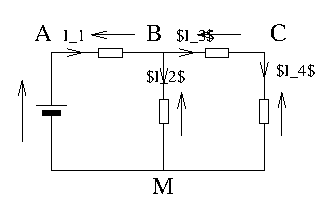
\includegraphics[width=7cm]{ds_2005_2006_term_stl_b/ds1/ex1_montage.eps}
\end{center}

%\begin{figure}[H] %[htbp]
%\begin{center}
%\input{ds_2005_2006_term_stl_b/ds1/ex1_montage.pstex_t}
%\caption{Montage 1}
%\label{figure:example}
%\end{center}
%\end{figure}


\begin{enumerate}

\item Annoter (avec les points $A$, $B$, $C$, $M$) les diff�rentes tensions.
\item \'Etablir les relations entre les diff�rentes intensit�s du courant.
\item \'Etablir les relations entre les diff�rentes tensions dans les mailles MBCM et MABM.

\end{enumerate}

\end{multicols}

\end{exercice}



%\newpage

\vspace*{\stretch{2}}

\begin{exercice} % ex1_montage

\begin{multicols}{2}



\begin{center}
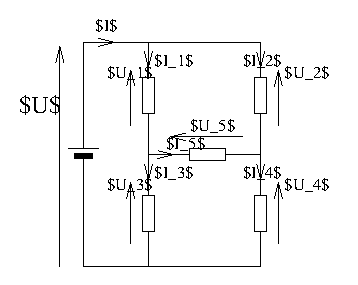
\includegraphics[width=7cm]{ds_2005_2006_term_stl_b/ds1/ex2_montage.eps}
\end{center}


\begin{enumerate}
\item Calculer les intensit�s des courants $I$, $I_3$ et $I_4$.
\item D�terminer les tensions $U_1$, $U_2$ et $U_5$.
\end{enumerate}


\donnees{
\item $U = 20~V$ ; $I_1 = 3~A$ ; $I_2 = 4~A$ ; $I_5 = 1~A$ ; $U_3 = 5~V$ ; $U_4 = 12~V$
}

\end{multicols}

\end{exercice}





\newpage

\vspace*{\stretch{2}}


\begin{exercice}

\begin{multicols}{2}

\begin{center}
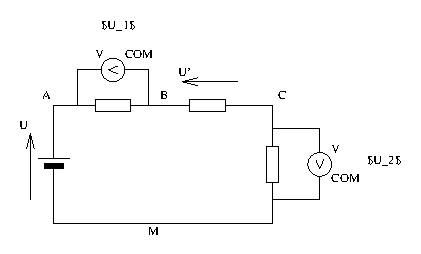
\includegraphics[width=7cm]{ds_2005_2006_term_stl_b/ds1/ex3_montage.eps}
\end{center}

Dans le montage ci-dessous les indications des voltm�tres sont les suivantes : $U_1 = 5~V$ et $U_2 = -10~V$.

Sachant que la tension aux bornes du g�n�rateur est $U = 20~V$, calculer $U'$.


\end{multicols}


\end{exercice}


\vspace*{\stretch{2}}


\begin{exercice}
On associe une r�sistance $R_1$ en s�rie avec deux r�sistances $R_2$ et $R_3$ associ�es en parall�le. On applique une tension $E$ � l'ensemble.


\begin{enumerate}
\item Faire le sch�ma du montage.
\item D�terminer l'intensit� du courant traversant $R_1$.
\item Calculer la tension $U_{R_1}$ aux bornes de $R_1$.
\item Calculer la tension $U_{R_{23}}$ aux bornes de $R_2$ et $R_3$.
\item Calculer l'intensit� du courant traversant $R_2$.
\item Calculer l'intensit� du courant traversant $R_3$.
\end{enumerate}


\donnees{
\item $R_1 = 56~\Ohm$ ; $R_2 = 68~\Ohm$ ;  $R_3 = 82~\Ohm$ ; $E = 6~V$
}

\end{exercice}


\vspace*{\stretch{2}}

\begin{exercice}
Un g�n�rateur r�el ($E$, $r$) est associ� en s�rie avec deux r�sistances $R_1$ et $R_2$.

\begin{enumerate}
\item Comment s'appellent $E$ et $r$ ?
\item Faire le sch�ma du montage.
\item Calculer l'intensit� du courant $I$ � l'aide de la loi de Pouillet (ou de la loi des mailles et la loi d'Ohm).
\end{enumerate}

\donnees{
\item $E = 12~V$ ; $r = 5~\Ohm$ ; $R_1 = 100~\Ohm$ ; $R_2 = 220~\Ohm$
}

\end{exercice}

\normalsize

\vspace*{\stretch{2}}

